\section{Background information} \label{background}
This section presents a brief overview of the inner workings of Docker and explores the technical details of the selected overlay solutions. Moreover, the GÉANT Testbeds Service environment is introduced.  

\subsection{Docker containers \& networking}
Docker is an open platform which aims to make building, shipping (portability), and running distributed applications easier \cite{docker2015}. In order to do so the applications are packaged in a 'container'. A Docker container functions as an execution environment and includes all of the dependencies and libraries required for the application to run. Each container follows a layered model in which layers are added on top of a base image as changes are made to the container. Figure \ref{fig:docker_layers} illustrates an example of this layered structure. On top of the read-only layers a thin read-write layer is shown. Any time a change is made to the running container, the changes are written to this read-write layer. After all changes have been made, the layer can be committed, which creates a new Docker \textit{image}. At that point, new containers can be deployed from the same image. Each container would have the same configuration and state as the container which was used to create the image. Committing layers to an image follows a similar principle as many version control systems employ. 

\begin{figure}[!ht]
   \centering
   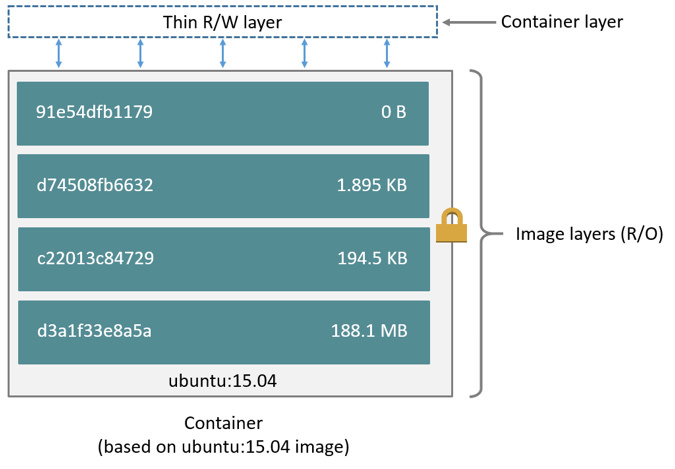
\includegraphics[scale=0.6]{img/container-layers.jpg}
   \caption{Layered model employed by Docker containers \cite{docker2015}}
   \label{fig:docker_layers}
\end{figure}

As with traditional virtualization techniques, containers allow for running multiple isolated user space instances on a single host. However, unlike traditional VMs, they don't require a hypervisor layer to be active on the host machine and instead directly share the kernel with the host machine. \cite{turnbull2014docker}. Furthermore, containers exclusively contain the necessary files to run. This inherently means that containers are lightweight and can start almost instantly. Because containers are so quick to deploy, and because they are deployed in a 'standardized' container format, they lend themselves to building extensive microservices consisting of a multitude of independent building blocks. 

Figure \ref{fig:workflow_docker} illustrates a generic workflow for deploying an application in a container. In the figure, the Docker host is responsible for hosting the containers and maintaining the images. By using the Docker client, the Docker daemon can be instructed to pull an image from the Docker registry. This registry is a centralized repository hosted by Docker, containing a large collection of official Docker images. This application can be a pre-packaged application image, which in turn can directly be deployed in a new container.

\begin{figure}[!ht]
   \centering
   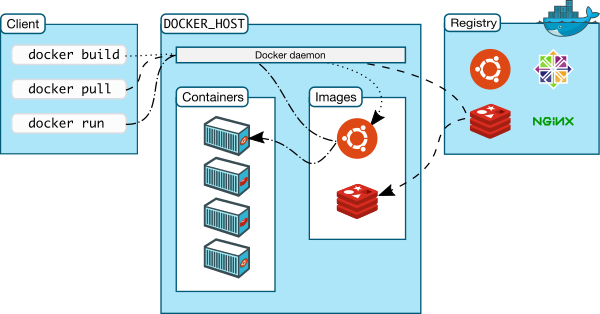
\includegraphics[scale=0.45]{img/architecture.png}
   \caption{Workflow for deploying applications to Docker containers \cite{multihost2015}}
   \label{fig:workflow_docker}
\end{figure}

The image illustrates how a Redis application is deployed in a single Ubuntu container. Docker was originally developed to improve the application development process. Docker allowed developers to build an entire multi-tier application on a single Linux workstation without the complexity or overhead of multiple operating system images \cite{techrepublic2015}. Because all containers were initially hosted on a single machine, Docker used a rather simple networking model. By default, Docker used private networking to connect containers via a special virtual bridge, \texttt{docker0}. This bridge was allocated a subnet from a private IP range. In turn, every deployed container was given a virtual Ethernet interface (usually abbreviated to 'veth' interface) which was attached to the \texttt{docker0} bridge. From inside of the container, the veth interface appeared as a regular \texttt{eth0} interface by using Linux namespaces. Each of the veth interfaces was addressed by the \texttt{docker0} bridge in the same private subnet. As a result, the containers were able to communicate with each other when they were located on the same physical machine and shared the same bridge interface. Prior tot Docker version 1.9, communicating with containers on other hosts was difficult. In order for the containers to communicate with each other they had to be allocated a static port on the hosting machine's IP address. This port number was then forwarded to other containers. Inherently this meant that hosting a cluster of web servers on a single node was difficult, as ports were statically mapped to specific containers. Connecting containers required a lot of coordination and planning. 

By linking containers with static ports, the overall configuration used to be relatively static. Moving containers between hosts required reconfiguration and portability was limited. Third party overlay projects were aiming to alleviate system administrators from static network configurations by connecting the containers via an an allocated IP address in an overlay network. Overlay networks allow for dynamically creating logical links between endpoints which have no coupling to the hardware infrastructure of the underlay network, effectively abstracting out the physical network. This meant that all containers in the overlay network could communicate with each other, regardless of their host placement or the IP address of the host machine. As such, containers do not have to be statically linked anymore based on a port number. However, early overlay solutions had to wrap around the Docker API as multi-host networking was not supported out of the box.

\subsection{Libnetwork}
The Docker team recognized the problem of connecting containers and as of version 1.9, \texttt{libnetwork} is included in the main release of the project. The idea behind \texttt{libnetwork} is to replace the networking subsystem that was in place in previous versions of the Docker Engine with a model that allows local and remote drivers to provide networking to containers. This means that Docker’s full networking code has now been included in a separate library called “\texttt{libnetwork}”. Docker achieved their modular ideal by implementing the Container Network Model (CNM). The premise of the CNM is that containers can be joined to networks in a multitude of ways and based on their configuration, all containers on a given network can communicate with each other \cite{5_bridgen_2015}. Previously, due to the static port bindings this proved to be difficult. With the introduction of CNM, Docker aims to address containers more like standalone hosts when they are deployed in overlay mode.

The innovation of the network stack was kickstarted when Docker acquired the SocketPlane team in March 2015 \cite{socketplane2015}. SocketPlane was one of the many available Software-Defined Networking solutions for containers on the market. Instead of connecting to a virtual bridge, each container would connect to an Open vSwitch (OVS) port. Each container host would have an OVS instance running which allowed them to form a virtual overlay network that would carry traffic destined for any container connected to the network via VXLAN. This allows containers to seamlessly communicate with each other wherever they are and thus enabling true distributed applications \cite{multihost2015}. 

\begin{figure}[!ht]
   \centering
   \includegraphics[scale=0.5]{img/cnm_model.png}
   \caption{Visual representation of the Container Network Model \cite{GITHUB}}
   \label{fig:cnm_model}
\end{figure}

The CNM relies on three main components: the sandbox, endpoints and networks. Figure \ref{fig:cnm_model} presents a visual representation of the three components placed in the model. In essence, the model is relatively simple. A (network) sandbox contains the configuration of a container's network stack. This includes management of the container's interfaces, routing table and DNS settings \cite{GITHUB}. As would be the case with a standard virtual machine, a sandbox can have multiple endpoints attached to a multitude of different networks. This is also illustrated in figure \ref{fig:cnm_model}. The middle container has two endpoints connected to two different networks. In turn, an endpoint connects a sandbox and thus a container to a network. A real world implementation of an endpoint could be a veth pair or in the case of various overlay solutions and Open vSwitch port for example. Docker defines a network in the CNM as "a group of Endpoints that are able to communicate with each-other directly" \cite{GITHUB}. An implementation of the network component could be a bridged network interface or a VXLAN segment.

Although Docker is the first containerization project to implement the model, CNM is a generic model that does not only apply to Docker exclusively, and can also be implemented in more traditional container projects like OpenVZ and LXC. By employing a modular model, \texttt{libnetwork} functions as a common ground for other overlay solutions. SocketPlane was only one of the available solutions on the market. Competing vendors and projects that can be identified are Calico, Flannel and Weave \cite{jorisclaassen2015}. As such there are many networking solutions available, suited for a large set of diverse use-cases. In order to standardize how containers are networked, \texttt{libnetwork} employs a driver plug-in model which allows third party solutions to plug directly into the Docker Engine. The end user on the other hand is only exposed to a consistent Network Model. The CNM abstracts the complexity of the third party plug-ins. For third party solutions, CNM provides a consistent programming interface which makes integrating with the Docker networking stack easier than in the past. 

The driver is the most abstract component of \texttt{libnetwork} and is not a user visible object. Drivers provide the actual implementation that makes the network work. By default Docker provides four drivers: a null, bridge, overlay and remote driver. The most commonly used driver is the 'bridge' driver. The bridge driver allows for single-host communication between containers by using Linux Bridging and iptables for segmentation. This driver is discussed in detail in Claassen's paper \cite{jorisclaassen2015}. The overlay driver is based on SocketPlane and implements networking that can span multiple hosts using VXLAN. Third party providers make use of the 'remote' driver. Build-in drivers such as 'bridge' and 'overlay' register inside of \texttt{libnetwork}, while remote drivers register with \texttt{libnetwork} via the plugin mechanism. 

\subsection{Third party overlay solutions}
During the course of this project we focus on the overlay solutions Calico, Flannel and Weave. Table \ref{overlayschar} presents a quick overview of the technical differences between the selected solutions. The successive subsections will to into more detail about each individual product.   

\begin{table}[H]
\centering
\begin{tabular}{@{}ll@{}}
\toprule
\textbf{Native overlay} & \textbf{Weave Net} \\ \midrule
Native integration & Libnetwork plug-in \\
VXLAN forwarding & VXLAN forwarding \\
Dedicated key-value store (any) & No dedicated key-value store (CRDT) \\
 &  \\ \midrule
\textbf{Flannel} & \textbf{Project Calico} \\ \midrule
No integration & Libnetwork Plugin \\
UDP or VXLAN forwarding & BGP routing \\
Dedicated key-value store (etcd) & Dedicated key-value store (any) \\ \bottomrule
\end{tabular}
\caption{Overlay solution characteristics}
\label{overlayschar}
\end{table}


\subsubsection{Weave}
Weave provides a Docker overlay solution named 'Weave Net'. Weave overlay consists of a multitude of Weave routers. Such a software router is placed on every machine participating in the overlay. In practice, this means a Weave container is launched within Docker. In addition to this container, a bridge interface is created on the host itself. In turn, containers within the overlay (including the Weave router) connect to this bridge using their veth interface which is supplied an IP address and subnet mask by Weave’s IP address allocator \cite{Weave2015}. As discussed in Section \ref{related}, Weave made use of \texttt{pcap} to route packets in previous versions of the project. However, as all packets had to be moved to userspace, this resulted in a significant performance penalty. In addressing this issue, Weave has added 'Weave Fast Datapath' in Weave version 1.2, which utilizes Open vSwitch \cite{davidwragg2015}. This allows Weave Net to do in-kernel routing which allows for significantly faster routing of packets between containers. Weave Router peers communicate their knowledge of the topology (and changes to it) to other routers, so that all peers learn about the entire topology. 

To application containers, the network established by Weave looks like a giant Ethernet switch to which all the containers are connected. In version 1.2, Weave was developed as a plug-in to \texttt{libnetwork}. As such, the Weave Net plugin actually provides two network drivers to Docker - one named \texttt{weavemesh} that can operate without a cluster store, and one named \texttt{weave} that can only work with one. By default \texttt{weavemesh} is utilized. As with all other overlays, Weave works alongside Docker's existing bridge networking capabilities which means that single-host communication is still possible without using Weave. In version 1.2, Weave still allows for \texttt{pcap} based routing when it is needed in specific scenarios. By default, Weave chooses their newly introduced Fast Datapath method (\texttt{fastdp}). However, when packets have to traverse untrusted networks and require encryption, the slower 'sleeve’ mode is used. At this point in time Weave can not provide encryption when using \texttt{fastdp} \cite{9_wragg_2015}.


%Weave creates a network bridge on the host. Each container is connected to that bridge via a veth pair, the container side of which is given an IP address \& netmask supplied either by the user or Weave’s IP address allocator. Also connected to the bridge is the weave router container. Weave routers learn which peer host a particular MAC address resides on. They combine this knowledge with topology information in order to make routing decisions and thus avoid forwarding every packet to every peer. Weave can route packets in partially connected networks with changing topology. Project Calico on the other hand utilises BGP for routing between containers and aims for extreme scalability.

%The topology information captures which peers are connected to which other peers. Weave peers communicate their knowledge of the topology (and changes to it) to others, so that all peers learn about the entire topology. This communication occurs over the TCP links between peers, using a) spanning-tree based broadcast mechanism, and b) a neighour gossip mechanism.

%Open vSwitch can operate both as a software-based network switch running within the virtual machine (VM) hypervisors, and as the control stack for dedicated switching hardware

%To application containers, the network established by weave looks like a giant Ethernet switch to which all the containers are connected.

%The Weave Net plugin actually provides two network drivers to Docker - one named weavemesh that can operate without a cluster store (like Docker’s overlay driver) and one named weave that can only work with one.

%Weave creates a virtual network that connects Docker containers deployed across multiple hosts and enables their automatic discovery. Weave works alongside Docker's existing (single host) networking capabilities, so these can continue to be used by containers.

%Fast data path reduces CPU overhead and latency because there are fewer copies of packet data and context switches. The packet goes straight from the user’s application to the kernel, which takes care of adding the VXLAN header (the NIC does this if it offers VXLAN acceleration).

%\begin{figure}[!ht]
%   \centering
%   \includegraphics[scale=0.42]{img/weave_userspace.png}
%   \caption{Weave datapath structure}
%   \label{fig:gts_env}
%\end{figure}

%In any case where Weave can’t use fast data path between two hosts it will fall back to the slower packet forwarding approach used in prior releases. The selection of which forwarding approach to use is automatic, and made on a connection-by-connection basis. So a Weave network spanning two data centers might use fast data path within the data centers, but not for the more constrained network link between them.

%Weave automatically chooses the fastest available method to transport data between peers. The most performant of these ('fastdp’) offers near-native throughput and latency but does not support encryption; consequently supplying a password will cause the router to fall back to a slower mode ('sleeve’) that does, for connections that traverse untrusted networks


\subsubsection{Flannel}
Flannel is another third party solution aimed towards building overlays between Docker hosts. The solution is part of CoreOS' product portfolio. Whereas Weave and Calico deploy separate container instances to manage the network, Flannel creates an agent, flanneld, on each container host which controls the overlay. All services are kept in sync via a key-value store.

The containers and their physical hosts are stored in the \texttt{etcd} datastore which is also created by CoreOS itself. Containers are assigned IP addresses from a pre-defined subnet, which is stored in the key-value store. Other than the alternative overlays, Flannel currently does not offer integration with the \texttt{libnetwork} plugin. However, representatives have noted it may very well be included later \cite{newsgroups_2015}. By default Flannel uses UDP tunneling to connect containers. In newer versions however VXLAN forwarding with Open vSwitch has been introduced to increase the performance of the overlay solution \cite{flannel_2015}.

As Flannel was built for Kubernetes, the solution  offers tight integration with the open source container cluster manager by Google. Kubernetes is aimed at large scale environments with a multitude of containers \cite{1_yakubovich_2014}.

\subsubsection{Calico}
Project Calico is technically not an overlay network but a pure layer 3 approach to virtual networking. Although we primarily evaluate overlay solutions, it is still worth mentioning because Calcio strives for the same goals as overlay solutions. The idea behind Calico is that data streams should not be encapsulated, but routed instead. This is achieved by deploying a BIRD Internet Routing Daemon on each container host. Calico uses the Border Gateway Protocol (BGP) as its control plane to advertise routes to individual containers across the physical network fabric \cite{calicosource}.

As with Flannel and Weave, every container is assigned its own IP address from a pre-defined pool. As Calico does not connect containers via tunneling techniques, segmentation between containers is achieved by modifying the \texttt{iptables} configuration of the host machine. Effectively, Calico functions as a firewall between network segments.

All traffic between containers is routed at layer 3 via the Linux kernel’s native IP forwarding engine in each host. This means that no overhead is imposed when containers try to communicate. No additional encapsulation headers are added. Like Weave, Calico functions as a \texttt{libnetwork} plug-in. The Calico network is controlled by a series of Docker containers, managed by the \texttt{calicoctl} tool which exchange state information via the BGP routing instances. State exchange of the network is achieved with BGP route reflectors

\subsection{Key value stores}
One dependency almost all overlay solutions share is the utilization of a Key-Value (KV) stores. This NoSQL datastore is used to create a key-value database to which the overlays technologies write their data. While the exact way the datastore is used differs slightly per overlay technology, generally the values stored are related to global IP address allocation and node discovery. In some cases additional information such as container names are also stored. Weave uses it's own proprietary storage system based on the 'Conflict-free Replicated Data Type' (CRDT) principle, as they believe this is best for the availability of the overlay \cite{7_richardson_2015}. The other technologies support a variety of KV-stores which are 'Consensus-Based' (CB). One example of an open-source CB datastore is \texttt{etcd}, which is the only datastore supported by all overlay technologies we will be using (Weave excluded). If any of the datastore-systems were to malfunction, the following effects would occur:

\begin{itemize}
  \item Inability to create new overlay networks;
  \item Inability to allocate global IP addresses;
  \item Inability to add a container to the overlay.
\end{itemize}

For the purposes of measuring the overlay performance, these implications are unrelated and not an issue. This is due to the fact that we are working with a fixed environment and are testing performance rather than availability.
Once the overlays and containers required for testing have been created and added to the KV store, the datastore will be idle. This means that the datastores used and their respective configurations are of no consequence to this project.

%\texttt{etcd} is a product of CoreOS

%Docker Networking in 1.9 requires an external Key-Value (KV) store, which is used for global IP address allocation and node discovery. The store is accessed via an API, libkv, that is advertised as working with Consul, etcd, and ZooKeeper.

%Essentially this means you have to install an additional distributed system in order to set up networking, for each Docker cluster, may not be to everyone’s taste. Scalability issues come into play when the amount of hosts in the KV store is extended beyond 5 to 10 hosts. Root cause analysis is harder: Figuring out whether bugs are in the application, or in Docker networking, or the external KV store, is up to you.

%Using the built-in network drivers in Docker 1.9 requires that a consistent KV store is visible from all Docker hosts. In practice however this either means a) having the KV cluster in one of the data centers, introducing a SPOF or b) spreading the KV cluster across multiple data centers, greatly increasing the likelihood of transient partitions and hence quorum failure (with results as above)

%All other Docker networking plugins, including Docker’s own “Overlay” driver, require that you set up Docker with a cluster store – a central database like Consul or Zookeeper – before you can use them. As well as being harder to set up, maintain and manage, every Docker host must be in constant contact with the cluster store: if you lose the connection, even temporarily, then you cannot start or stop any containers.

%All cross-host coordination is handled by Weave Net’s “mesh” communication, using gossip and eventual consistency to avoid the need for constant communication and dependency on a central cluster store.

\subsection{GÉANT Testbed Services} \label{gts_sec}
In order to do performance measurements in a realistic setting, which resembles a network distributed over the internet, the GÉANT Testbeds Service (GTS) will be utilized. This service offers the ability to create experimental networks at scale, geographically dispersed over five European cities. Figure \ref{fig:gts_env} presents a high-level overview of the GTS environment. GÉANT is a European research network which focuses on services aimed at research and education. GÉANT has Points of Presence (PoPs) in Amsterdam, Bratislava, Ljubljana, Milan and Prague. The sites are connected via dedicated point-to-point circuits 10 Gbps optical waves in an Multi Protocol Label Switching (MPLS) cloud.

The GTS physical infrastructure is assembled into a set of equipment pods which contain the hardware components that make up the virtual machines, virtual circuits and other resources. Figure \ref{fig:gts_env} presents a high level overview of the GTS infrastructure. All locations provide equal capabilities for provisioning (virtual) machines and provide equal connectivity. The virtual machines in GTS are deployed in Kernel-based Virtual Machine (KVM) by OpenStack. Each VM uses \texttt{pci\_passthrough}, giving it full and direct access to the network interface card (NIC) of the host machine. All virtual machines are deployed with Ubuntu 14.04 LTS by default.

\begin{figure}[!ht]
   \centering
   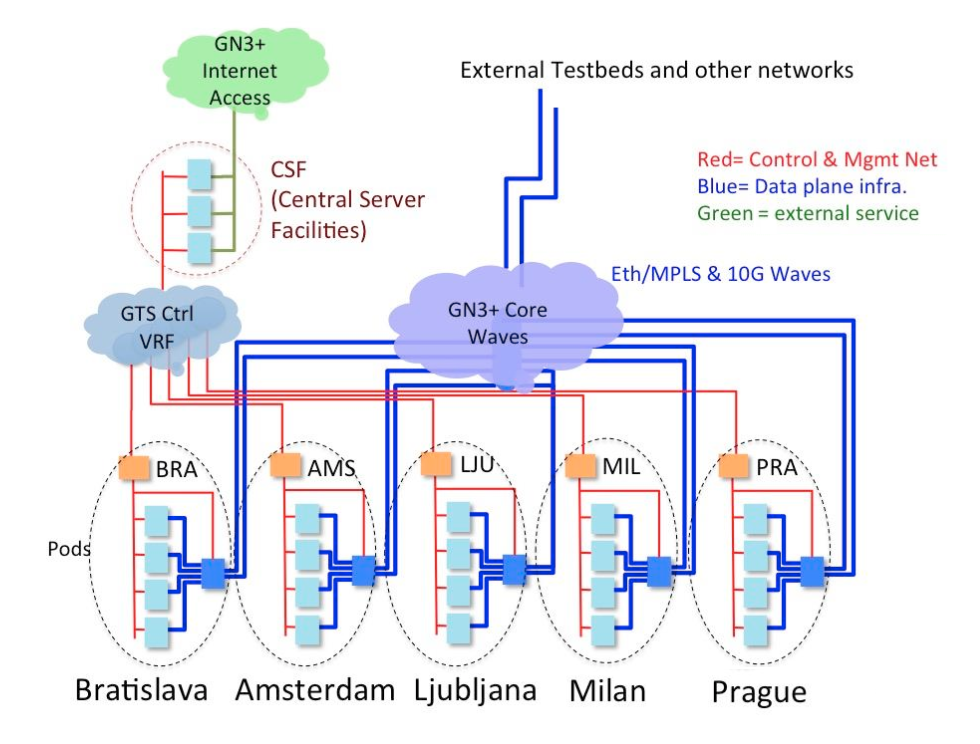
\includegraphics[scale=0.32]{img/gts_env.png}
   \caption{The GTS distributed architecture across the GÉANT core network}
   \label{fig:gts_env}
\end{figure}

Each testbed created in the environment forms an isolated (virtual) environment which shares resources with other users of the service. As such, interference with other projects running within GTS is to be expected and cannot (and should not, for the purposes of this project) be avoided. This way generic Internet traffic is resembled. Preliminary tests in the testbed service have shown latencies between the PoPs ranging between 15 ms and 60 ms which falls within our definition of high latency as presented in Section \ref{intro}.

